\documentclass[12pt]{ctexart}
\usepackage{extsizes}
\usepackage{amsmath}
\usepackage{geometry}
\usepackage{graphicx}
\usepackage{geometry}
\usepackage{color}
\usepackage{listings}
\usepackage{fontspec}
\usepackage{fancyhdr}
\usepackage[boxed,ruled,linesnumbered]{algorithm2e}
\usepackage{threeparttable}
\usepackage{float}
\geometry{a4paper, scale=0.8}
\graphicspath{ {../pics/} }
\definecolor{ngrey}{RGB}{77, 93, 83}
\definecolor{dkgreen}{rgb}{0,0.6,0}
\definecolor{gray}{rgb}{0.5,0.5,0.5}
\definecolor{mauve}{rgb}{0.58,0,0.82}
\pagestyle{fancy}
\newfontfamily\monaco{Consolas}
\fancyhead{}
\fancyhead[C]{同化棋实验报告\quad 梁博强}
\setcounter{section}{-1}
\lstset{ %
  language=python,                % the language of the code
  basicstyle=\footnotesize\monaco,           % the size of the fonts that are used for the code
  numbers=left,                   % where to put the line-numbers
  numberstyle=\scriptsize\color{gray}\monaco,  % the style that is used for the line-numbers
  stepnumber=2,                   % the step between two line-numbers. If it's 1, each line 
                                  % will be numbered
  numbersep=5pt,                  % how far the line-numbers are from the code
  backgroundcolor=\color{white},      % choose the background color. You must add \usepackage{color}
  showspaces=false,               % show spaces adding particular underscores
  showstringspaces=false,         % underline spaces within strings
  showtabs=false,                 % show tabs within strings adding particular underscores
  frame=shadowbox,                   % adds a frame around the code
  rulecolor=\color{gray},        % if not set, the frame-color may be changed on line-breaks within not-black text (e.g. commens (green here))
  tabsize=2,                      % sets default tabsize to 2 spaces
  captionpos=b,                   % sets the caption-position to bottom
  breaklines=true,                % sets automatic line breaking
  breakatwhitespace=false,        % sets if automatic breaks should only happen at whitespace
  title=\lstname,                   % show the filename of files included with \lstinputlisting;
                                  % also try caption instead of title
  keywordstyle=\color{blue},          % keyword style
  commentstyle=\color{dkgreen},       % comment style
  stringstyle=\color{mauve},         % string literal style
}

\begin{document}
	\title{同化棋: 一种基于蒙特卡罗树搜索的解决方案}
	\author{梁博强\quad 元培学院}
	\date{\today}
	\maketitle

	\begin{abstract}
		\normalsize
		在本学期计算概论课程的同化棋大作业中,笔者采用了一种基于蒙特卡罗树搜索(MCTS)的算法来实现
		并优化机器决策,并针对同化棋进行改进,最终取得了优于朴素贪心算法的成绩。
		本文将简要介绍这次大作业的设计思路、实现过程、决策优化、相关工作
		和后续进一步工作的方向。
	
		通过本次大作业的实践,我对各种主流的博弈算法有了初步了解。此外笔者将 C++ 实现的决策算法
		封装在动态链接库中,并搭建了与 Python 编写的图形界面框架的连接,这加深了我对程序之间交互的
		理解。而在实现程序具体功能、提高程序实用性的过程中,笔者对文件读写、面向对象编程、树数据结构、
		Tkinter 图形用户界面、异常处理等有了进一步认识。
	\end{abstract}

	\section{背景}

	\subsection{同化棋}
	同化棋(Ataxx),是Dave Crummack和Craig Galley在1988年发明,1990年出品于电视游戏而流行的两人棋类,可说是黑白棋的衍生。\footnote{https://en.wikipedia.org/wiki/Ataxx}
	其最主要的特点是落子后会将邻近八格的所有敌方棋子颜色翻转,并且原棋子有可能是被复制的,也有可能是被移动的。

	同化棋的上述特点为机器决策带来了难度: 相比于相同规模的其他常见棋类,从当前局面状态到下一局面状态的\textbf{决策分支}可能更多;当前状态与
	下一状态间的\textbf{局面估值}(value)的差可能较大,这就要求我们在蒙特卡罗树搜索算法的基础上加以改进。

	\subsection{蒙特卡罗树搜索}
	蒙特卡罗树搜索(MCTS)是一种用于某些决策过程中的启发式搜索算法,其核心思想是用随机抽样的方法来解决确定性问题,
	最早起源于20世纪40年代。\footnote{https://en.wikipedia.org/wiki/Monte\_Carlo\_tree\_search}1987年,Bruce Abramson 将游戏中的 minmax 搜索算法进行改进,他把静态估值函数替换成随机博弈展开的期望,
	并在黑白棋和象棋上取得了较好的成绩。

	2016年,AlphaGo 战胜了围棋职业选手李世石,名噪一时。 AlphaGo 将MCTS与两个神经网络(分别对局面和策略估值)结合,从而使得它的效率相较于传统的MCTS有了质的提升。

	MCTS 主要分为四个步骤:选择、扩展、模拟、反向传播,这四个步骤循环进行,使得统计结果逐渐接近真实情况。

	\begin{figure}[H]
		\centering
		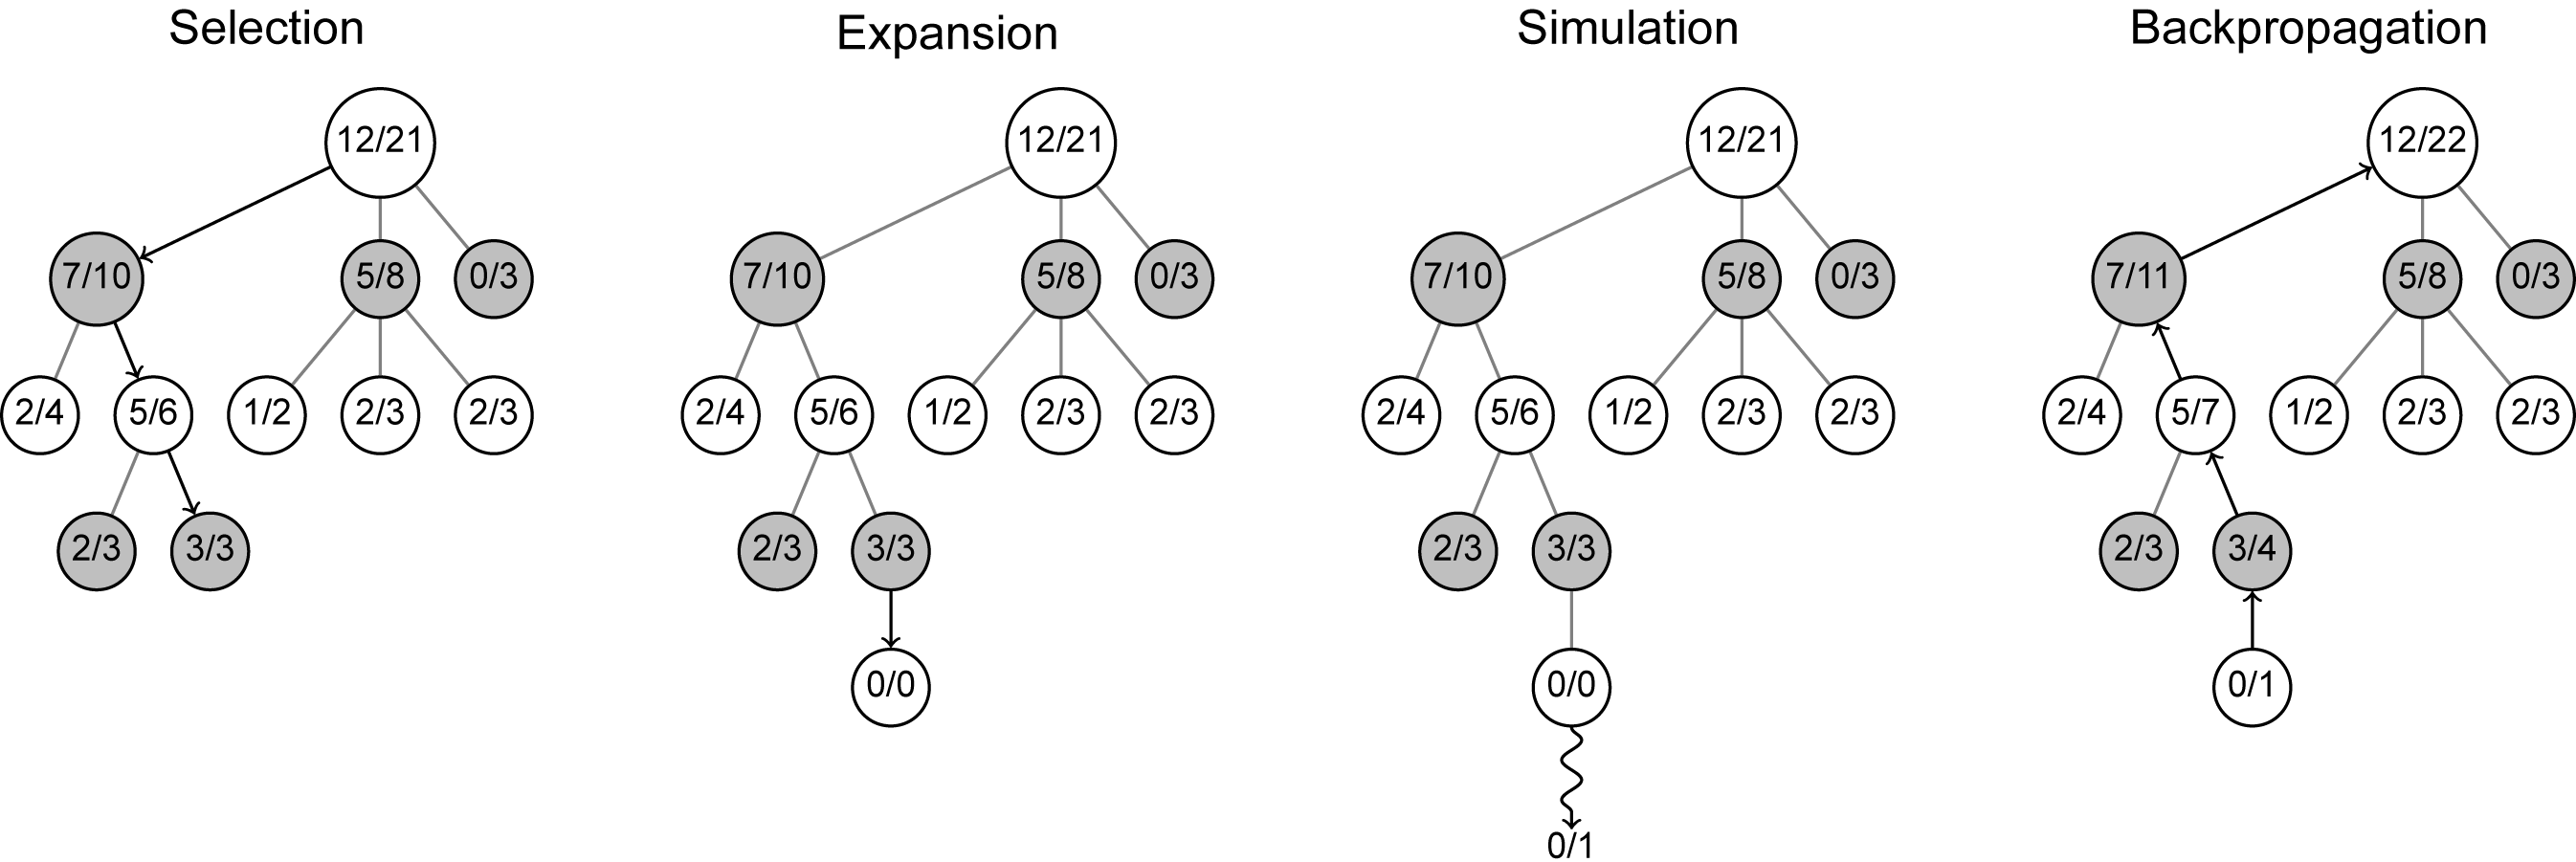
\includegraphics[width = 0.9\textwidth]{MCTS.png}
		\caption{MCTS的四个步骤图示}
	\end{figure}
	
	\subsubsection{选择(Selection)}
	从根节点$R$开始,连续向下选择子节点至叶子节点$L$。

	选择子节点的过程是MCTS的精髓所在。我们既希望探索胜率较高的节点,也希望兼顾那些被探索得较少的节点。
	第一个在游戏中平衡利用与探索的公式被称为UCT(Upper Confidence Bounds to Trees,上限置信区间算法)
	,其表达式为
	\[UCT = \frac{w_i}{n_i}+c\sqrt{\frac{\ln{N}}{n_i}}\]
	上式中,$w_{i}$代表第$i$次移动后取胜的次数;
	$n_i$代表第$i$次移动后仿真的次数;
	$c$为探索参数,理论上等于$\sqrt{2}$;在实际中通常可凭经验选择;
	$N$代表父节点模拟总次数,即$\sum n_i$。

	\subsubsection{扩展(Expansion)}
	如果游戏在叶节点$L$还没结束,创建新的子节点并选择其中一个节点$C$。

	\subsubsection{模拟(Simulation)}
	从新的叶节点$C$开始,用随机策略进行游戏,又称为 playout 或 rollout。

	\subsubsection{反向传播(Backpropagation)}
	使用随机游戏的结果,更新从$C$到$R$的路径上的节点信息。
	
	\section{MCTS 算法实现与优化}

	\subsection{数据结构}
	每个蒙特卡罗树节点包含当前局面、执子者颜色、父节点指针、搜索深度、节点被访问的次数以及反向传播的估值总和。
	每个节点用一个优先队列记录它的子节点指针,排序规则是下个节点的 UCT 估值更大的在前;如果两个节点 UCT 估值相同(比如说两个节点都没被探索时)
	我们取当前执子者看来“相对得分”更优的子节点在前。

	相对得分(代码中定义为\textsf{relscore})即为黑白节点数之差,其正负是由当前节点的着子颜色决定。

	同时,为了减少搜索次数,特地增加了一些标记表明该节点是否有必胜策略,如果有,则直接开始逆向传播过程即可。

	\subsubsection*{空间压缩的尝试}
	我们用两个49位的位向量来表示当前局面,第一个位向量中为1的位表示当前位置有白子,同理第二个位向量表示哪里有黑子。
	这样我们将一个局面占用的空间压缩到了16字节。同时,因为在找出最佳字节点后我们要求出怎么走才能达到它,我们也用一个位向量表示一步走棋。
	用4个3位的空间分别表示选择的棋子和落子位置的横纵坐标,用一位表示这个走法是哪个类型的。

	\subsection{选择环节估值函数}
	在估值函数的实现,我基于UCT函数,针对同化棋的特性做了细微的更改,首先如果节点未被访问过,那么我们将它的估值设为一个极大值,这样我们可以
	保证未被探索的子节点都排在子节点表(优先队列)的前面,选择时可无需特意挑选未被拓展过的子节点。

	如果子节点被访问过,那么我们的估值函数如下式:
	\[UCT'= - \frac{\sum val}{vis} + c_0\sqrt{\frac{\ln(N)}{vis} }- c_1\times relscore - c_2\times step.type\]
	上式中$val$是某一次反向传播回的估值,需要注意的是父节点总倾向选择子节点得分最少的情况;$vis$是节点被访问的总次数。

	$relscore$是当前局面的“相对得分”,加入这一项的想法来自于贪心算法,在搜索次数不是很多,各节点估值在统计上不太有代表性的时候,
	可以通过贪心“指导”MCTS更倾向下一步决策最优。当决策次数变多时,这个项的占比就相对变低了

	$step.type$是这一步走棋的类型,实验证明,让MCTS选择“复制粘贴”型落子往往略好于“剪切复制”型,这项占比是最小的,同样地,这也是搜索次数较少时的一种“指导”。

	$c_0,c_1,c_2$是正的常数,通过实验不断优化。

	\subsection{模拟环节的实现}
	在模拟环节,由于同化棋随机走法与真实局面的误差过大,我采用贪心的算法来提高模拟的精确度,即求出所有的情况,选出“相对得分”(\textsf{relscore})最优的子节点。
	但这样做牺牲了随机算法的高效性。
	经过试验,我们确定了 MCTS 的最大模拟深度大约从根结点开始的30-50回合。简单地,我们采用最后节点的“相对得分”作为反向传播用的估值。
	如果在达到我们设定的最大模拟深度之前,游戏提前达到终局,那么我们会按线性放大这个估值。
	这样做既是为了奖励 MCTS 算法采用更为激进的决策提前赢得游戏,也是因为模拟到终局时结果往往更加精确。

	\begin{algorithm}
		\caption{模拟阶段node::simulation()}
		\SetKwFunction{ex}{expand}
		\SetKwFunction{sm}{simulation}
		\SetKwData{v}{value}
		\SetKwData{ch}{choice}
		\SetKwData{cq}{childqueue}
		\KwOut{back prop \v}
		\ch $\gets$ \cq .top()\;
		\If{\ch not expanded}{\ex {\ch}}
		\If{\ch game terminates}{
			\v -= \ch$\rightarrow relscore\times f(depth)$\;
			\KwRet{-\ch$\rightarrow relscore\times f(depth)$}}
		\Else{
			\v += \ch$\rightarrow$\sm\;
			\cq .pop()\;
			\cq .push(\ch)\;
			\Return{-\ch$\rightarrow$\sm}}
		
	\end{algorithm}
	

	\section{用户端功能实现}
	\subsection{源文件组织结构}
	源代码文件(见附件)的相互关系如图2所示。 \textsf{gui.py} 是程序与用户交互的图形界面,\textsf{core.py} 中有python下基本的同化棋游戏类,定义了游戏的基本规则、局面状态,以及存盘、读盘、悔棋等操作的实现。
	\textsf{core.py} 通过调用动态链接库\textsf{mcts.dll}(源代码是 \textsf{mcts.cpp} ,有 MCTS的数据结构)中封装好的决策函数,输入当前局面,得到 MCTS 给出的走法。\textsf{mcts-short.cpp}是笔者提交到 botzone 上的版本,不同点在于内置了对 botzone 上 json 输入输出的解析。
	save文件夹里存有玩家的存档文件。

	\begin{figure}[H]
		\centering
		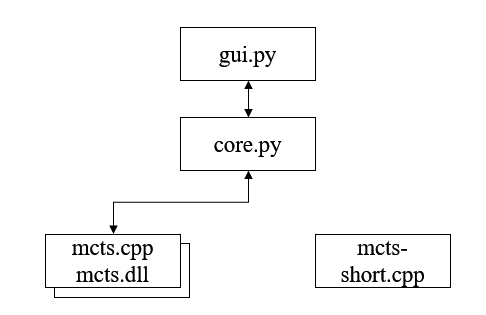
\includegraphics[width = 0.5\textwidth]{graph.png}
		\caption{源文件间组织关系}
	\end{figure}

	\subsection{图形用户界面(GUI)}
	笔者采用python中的tkinter来绘制图形界面。包含有五个功能(新游戏、保存、读取、悔棋、退出)的功能按钮、当前比分,以及用图片叠加绘制的棋盘。游戏时,玩家选中的棋子会被高亮显示,落子后,棋盘会被更新。

	由于同化棋每次落子时需要进行两次点击,且两次点击的处理方式有所不同,笔者定义了两个函数 \textsf{handler1}, \textsf{handler2},轮流作为点击画布(\textsf{<Button-1>})这一行为的信号处理函数。当游戏结束且新游戏未开始时,程序不处理画布点击的信号。
	当程序准备好接受用户输入时,信号处理函数设为 \textsf{handler1} ,点击画布时,\textsf{handler1} 判断选子位置是否合法,若是,则记录被点击的我方棋子,将选中棋子高亮,然后将\textsf{handler2}设为点击画布的信号处理函数。

	\textsf{handler2} 接下来会负责处理第二次点击动作,如果第二次点击也是合法的,我们执行落子,更新棋盘,这之后就不处理点击画布的信号,此时我们调用机器决策的函数,待机器决策完成后更新画布,
	如果棋局没有终结,则将信号处理函数设为\textsf{handler1},接收新的点击信号,否则我们应该继续屏蔽所有对画布的点击。

	代码如下:
	\newpage

	\begin{lstlisting}
def handler(self,e):
	x0 = int(e.x//50)
	y0 = int(e.y//50)
	if self.playing.invalid(x0,y0):
		return

	self.selected=x0,y0
	self.cic = self.board.create_image(x0*50+25,y0*50+25,image=self.image[human_color])
	self.board.bind("<Button-1>", self.handler2)

def handler2(self,e):
	self.board.unbind("<Button-1>")
	x1 = int(e.x//50)
	y1 = int(e.y//50)
	x0,y0 = self.selected
	if self.process_invalid(x0,y0,x1,y1):
		self.board.delete(self.cic)
		self.board.bind("<Button-1>", self.handler)
		return

	self.playing.proceed(-self.playing.bot_color, x0,y0,x1,y1)
	self.playing.js['requests'].append({'x0':x0, 'y0':y0, 'x1':x1, 'y1':y1})
	self.drawings()

	if self.playing.dead(): 
		self.handel_death()
		return

	self.some_buttons.config(state=DISABLED)
	self.playing.bot_decision()
	self.some_buttons.config(state=NORMAL)
	self.drawings()
	
	if self.playing.dead():
		self.handel_death()
		return
	self.board.bind("<Button-1>", self.handler)
	\end{lstlisting}

	\subsection{保存、读取与新游戏}
	对于存档文件的设计,我采用和botzone上输入一样的json字符串来存储一个局面,即记录双方每一次走棋的源棋子和落子点。

	开始新游戏时我们直接创建一个新的\textsf{game}类,并执行初始化。若要读取存档,我们就会按照存档json文件中的走棋记录,
	重新演绎这个局面。

	\subsection{悔棋}
	采用json(在局面运行时实际上是Python中的词典数据结构)记录局面虽然会使存盘占用空间更大,读盘更加复杂,但好处是我们可以实现任意多步的悔棋。
	具体来说,我们会删除上一次双方的走棋记录,然后进行类似于创建新游戏的过程,但我们只会演绎到棋局的倒数第三步。

	\section{结果}
	本文的算法取得了优于贪心算法的成绩,与贪心算法的AI对弈10局,本算法取得了8胜2负的成绩。

	在botzone平台上,本文算法的排位分目前是1010分\footnote{botzone bot id: 61d57acc8d8bd011d7838b50},在班级正式赛中,本算法同样排位在中游水平。

	GUI程序连同MCTS算法都没有任何导致崩溃或错误的恶性bug。

	\section{不足与后续工作}
	必须承认,笔者完成这份作业较为仓促,因此仍有很多地方有待改进。

	\subsection{MCTS探索节点数较少}
	尽管笔者尝试采用限制展开环节的深度,以及用叶节点的局面的估值(棋子数之差),但在规定时间内所能
	探索的节点数仍然较少,仅达到1000个左右。而同化棋中,每个状态节点对应的子节点约有10-100个,MCTS要求我们完成展开的次数应明显高于
	每个节点的子节点数,才能实现较好的决策。

	反映在结果中,我们可以看到本算法在对局开始(前15回合)和结尾(后15回合)时的决策明显优于中期的决策。
	原因可能是在对局前期,决策算法会倾向于先复制并占领更多的空白,或是试图在搜索深度限制内吃掉对方所有棋子。
	在对局末期,MCTS几乎能枚举到所有最可能被打出的决策,从而给出精确的最优决策。但在对局中期,MCTS很难模拟展开到终局,
	使得节点的估值很不精确。

	探索节点数较少的原因可能在于: 首先,同化棋的决策分支数相对较多。更重要的是,采用贪心算法,而非随机决策进行展开模拟虽然可以获得比较好的模拟结果,但是对于每一个局面
	我们需要枚举所有可能的落子决策,这极大增加了算法的时间复杂度。

	后续我们可以进一步优化不同回合时MCTS展开的深度限制,使得我们在“探索更多节点”与“模拟到更多终局”间取得一个平衡。另外,我们可以优化展开时的贪心算法,从所有移动方法为“复制”
	的落子决策中取得最优解;抑或是用叶节点的局面估值代替模拟展开结果,这样都能减少模拟展开时的时间复杂度。
		

	\subsection{搜索树未被长时保留}
	在 Botzone 平台上运行以及线下提交的版本中,笔者采用的都是常见的短时运行方式,即每一次决策结束后退出搜索
	函数,同时清空搜索树。这样做的稳定性较高,但每一次决策时都要重新构建搜索树。有趣的是,MCTS最终选择的子节点是我们探索次数最多的
	节点,往往有最多已探索的后代节点,重新探索、模拟、展开这些后代节点会造成很大浪费。

	保留搜索树、采用长时运行模式并不难,但关键是决策后需要清理其他的分支节点,避免造成内存浪费。否则,经过数轮决策,搜索树
	的大小会显著超过Botzone上的内存限制。因此也有必要优化数据结构,减小单个节点占用的空间。

	\section{总结}
	通过本次大作业的实践,我对各种主流的博弈算法,包括minmax,及$\alpha-\beta$剪枝,甚至是深度学习方法有了初步了解。此外我对多文件编程以及程序之间交互的
	理解。而在实现程序具体功能、提高程序实用性的过程中,我对文件读写、面向对象编程、树数据结构、
	Tkinter 图形用户界面、异常处理等有了进一步认识。

	而编写AI参与比赛的经历也提醒着我,设计一个发达的智能体是一件可以精益求精,一直钻研下去的事情;扎根于某一领域深入探究,也是别有乐趣的。

	
\end{document}